\section{Распределения данных}

\subsection{Отбор данных}
\begin{terms}
    \item[Генеральная совокупность (population)] Полный наблюдаемый набор данных.
    \item[Выборка (sample)] Подмножество набора данных.
    \item[Репрезентативная выборка] Достоверно представляет всю популяцию в целом.
    \item[Смещение (bias)] Систематическая ошибка отбора.
    \item[Смещенная выборка] Представляющая популяцию в искаженному виде.
    \item[Случайный отбор] При котором каждый элемент имеет одинаковую вероятность попасть в выборку.
    \item[Простая случайная выборка] Результат случайного отбора.
    \item[Страты] Множество элементов с некоторым схожим признаком.
    \item[Стратифицированный отбор]
    Разделение генеральной совокупности на страты и случайный отбор элементов из каждой страты.
\end{terms}
Случайный отбор может производиться как с возвратом элементов, так и без него.
\par Качество данных часто имеет большее значение, чем их количество.

\subsection{Выборочное распределение статистики}
\begin{terms}
    \item[Выборочная статистика] Метрический показатель для выборки.
    \item[Распределение данных] Частотное распределение значений в наборе данных.
    \item[Выборочное распределение] Частотное распределение выборочной статистики на выборках.
    \item[Центральная предельная теорема] Тенденция выборочного распределения принимать нормальную форму
    по мере увеличения размера выборок.
    \item[Стандартная ошибка] Изменчивость выборочной статистики на выборках.\\
    $\sigma / \sqrt{n}$, \quad \sigma --- стандартное отклонение.
\end{terms}

\subsection{Бутстрап}
\begin{terms}
    \item[Бутстрап] Взятие выборки с возвратом из популяции.
    \item[Повторный отбор (resampling)] Бутстрап с перестановками.
\end{terms}
\textbf{Применения бутстрапа:}
\begin{itemize}
    \item Определение вариабельности выборочной статистики.
    \item Работа с выборками без использования математических приближений.
    \item Оценка выборочных распределений для статистик.
    \item Бэггинг (Bootstrap aggregating): агрегирование предсказаний.
    \item Создание доверительных интервалов.
\end{itemize}

\subsection{Доверительные интервалы}
\begin{terms}
    \item[Доверительный интервал] С заданной вероятностью накрывает оцениваемый параметр популяции.
    \item[Уровень значимости] Вероятность непопадания значения в доверительный интервал.
    \item[Уровень доверия] Вероятность покрытия интервалом значения.
\end{terms}

\subsection{Нормализация}
\begin{terms}
    \item[Нормализация] Преобразование данных к безразмерным единицам в рамках заданного диапазона
    или с заданным свойством.
    \item[Стандартизация] Преобразование исходного набора в новый с $\overline{x} = 0$ и $\sigma = 1$\\
    \begin{equation*}
        z = \frac{x - \overline{x}}{\sigma}
    \end{equation*}
    \item[Минимакс] Преобразование исходного набора в диапазон $[0, 1]$.
    \begin{equation*}
        x_{norm} = \frac{x - x_{min}}{x_{max} - x_{min}}
    \end{equation*}
\end{terms}
Ключевая цель нормализации --- приведение данных к единому виду,
который позволит сравнивать их между собой или использовать для расчёта схожести объектов.

\subsection{Распределения}
\begin{terms}
    \item[Квантиль-квантильный график (QQ-plot)] Показывает связь между наблюдаемыми значениями
    и стандартизированными квантилями. %TODO
    %TODO add info about distributions
\end{terms}
В нормальном распределении 68\% данных находятся в пределах одного
стандартного отклонения от среднего и 95\% — в двух стандартных отклонениях.\\
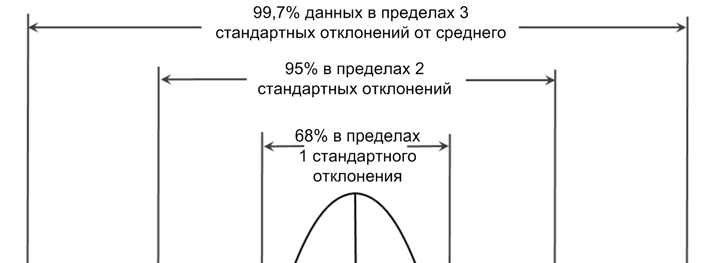
\includegraphics[scale=0.5]{50 notions/img/norm_dist1}\\
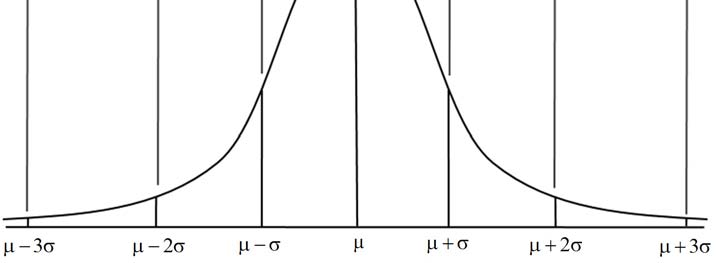
\includegraphics[scale=0.5]{50 notions/img/norm_dist2}